\documentclass[10pt, a4paper]{article}

\usepackage[english]{babel}
\usepackage{polski}
\usepackage[utf8]{inputenc}
\usepackage{graphicx}
\usepackage{float}
\title{Rozwiązanie zadania 3 z zestawu 3 z "Projektowania obiektowego oprogramowania"}
\author{Mateusz Małowiecki}
\begin{document}
\maketitle
\section*{Polecenie}
Dokonać analizy projektu obiektowego pod katem zgodności klasy CashRegister z zasadą OCP. Zaproponować takie zmiany, które uczynią ją
niezmienną a równocześnie rozszerzalną jeśli chodzi o możliwość implementowania różnych
taryf podatkowych oraz drukowania paragonów z uwzględnieniem różnego porządkowania
towarów (alfabetycznie, według kategorii itp.)
Narysować diagramy klas przed i po zmianach. Zaimplementować działający kod dla przykładu przed i po zmianach demonstrując kilka różnych rozszerzeń.
\begin{verbatim}
public class TaxCalculator {
   public Decimal CalculateTax( Decimal Price ){
       return Price * 0.22 
   }
}
public class Item {
   public Decimal Price { get { ... } }
   public string Name { get { ... } }
}
public class CashRegister {
   public TaxCalculator taxCalc = new TaxCalculator();
   public Decimal CalculatePrice( Item[] Items ) {
       Decimal _price = 0;
       foreach ( Item item in Items ) {
           _price += itemPrice + taxCalc.CalculateTax( item.Price );
       }
       return _price;
}
public string PrintBill( Item[] Items ) {
   foreach ( var item in Items ) {
       Console.WriteLine( "towar {0} : cena {1} + podatek {2}", item.Name, item.Price, 
       taxCalc.CalculateTax( item.Price ) );
   }
}
\end{verbatim}
\section*{Rozwiązanie}
\subsection*{Dokonać analizy projektu obiektowego pod katem zgodności klasy CashRegister z zasadą OCP.}
Klasa CashRegister łamie zasadę OCP, ponieważ nie jest otwarta na rozszerzenia. Korzysta ona z konkretnej implementacji TaxCalculator i nie ma możliwości, żeby mogła ona wyliczać podatek w inny sposób. Dodatkowo drukowanie paragonów jest zaimplementowane bezpośrednio w klasie CashRegister, w wyniku czego nie mamy wymienności implementacji drukowania. Jeszcze jednym problemem jest to, że klient jest uzależniony od konkretnej implementacji klasy Item, a powinien mieć możliwość dodać własną implementację tej klasy.
\subsection*{Zaproponować takie zmiany, które uczynią ją niezmienną a równocześnie rozszerzalną jeśli chodzi o możliwość implementowania różnych taryf podatkowych oraz drukowania paragonów z uwzględnieniem różnego porządkowania towarów (alfabetycznie, według kategorii itp.)}
Proponowane zmiany: \\
1. Dodanie nowego interfejsu ITaxCalc z metodą CalculateTax (abstrakcja klasy TaxCalculator). \\
2. Dodanie nowego interfejsu IItem z polami Price i Name (abstrakcja klasy Item). \\
3. Dodanie interfejsu IItemSort odpowiedzialnego za sortowanie elementów. \\
4. W konstruktorze klasy CashRegister inicjujemy taxCalc obiektem klasy implementującej interfejs ITaxCalc.
\subsection*{Narysować diagramy klas przed i po zmianach.}
Diagram przed:
\begin{figure}[H]
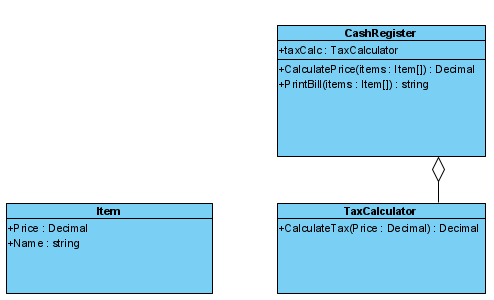
\includegraphics{Diagram_before}
\end{figure}
Diagram po:
\begin{figure}[H]
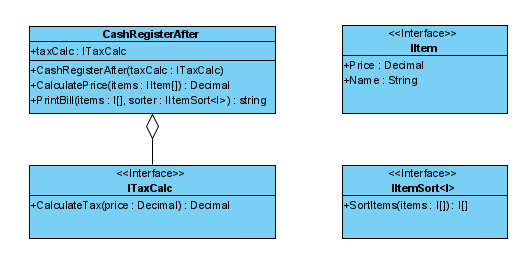
\includegraphics{Diagram_after}
\end{figure}
\subsection*{Zaimplementować działający kod dla przykładu przed i po zmianach demonstrując kilka różnych rozszerzeń.}
Kod znajduje się w plikach "POO\_L3\_Z3\_After.cs" i "POO\_L3\_Z3\_Before.cs". W pliku "POO\_L3\_Z3\_Test.cs" znajdują się testy.
\end{document}